The following literature review explores mesh networks in a wooded area,
	when communicating from two devices across a network there are a lot of issues associated with this communication
	such as signal loss due to:
	\begin{itemize}
		\item Environmental conditions such as rain .lighting etc
		\item If the device's antenna is in line of sight with each other
		\item Even if the devices are in the line of sight we can still reflections from a multi-path environment
		\item Possibility of trees falling obstructing the path of the signal causing more attenuation in the signal strength
	\end{itemize}
	In this project I want to explore mesh networks and transmit data across them,  a mesh network is a type of network where no node(a node is just a device which has a transceiver ) in the network acts as a  master.
	As we look at the environment in which this project aims to be, we expect different phenomena to occur such as  Attenuation According to ITU \cite{ITU} "attenuation due to vegetation varies widely due to the irregular Nature of the medium and the wide range of species, densities and water content obtained in practice"
	when transmitting any radio wave it takes energy another factor to consider is whether wind which will cause a  delay in the signal. this report aims to show my findings and try to count for Environmental conditions
	\subsection{Overview} \label{sec: overview}

		This section provides a brief overview of  my project on mesh networks in a forest the following question is:
		
		\begin{enumerate}
			\item What frequencies can transmit in a forest
			\begin{itemize}
				\item What are the Disadvantages of transmitting at this range
				\item What are the effects of the multi-path environment when there is a line of sight
				\item What happens to Non-line of sight
			\end{itemize}
			\item What sensors /senor modules do we use
			\begin{itemize}
				\item What sensors will give us a good range in an Irish forest
				\item What are the limitations on the board we use
				\item Do we need to  have any additional hardware to  accommodate a specific board 
			\end{itemize}
			\item What microprocessor/hardware do we use?
			\begin{itemize}
				\item What advantages/Disadvantages of  Arduino vs Raspberry Pi
				\item What is the major factor in the choice 
				\item How are the sensors wired to the processor 
				\item How to read the  data
				\item What is the effective Resolution needed for each application
			\end{itemize}
			
		\end{enumerate}
	\newpage
	\subsection{Mesh network}
	A mesh network is a type of network that uses multiple devices to relay data between each other, making a decentralized network
	the mesh we looking to use is a wireless mesh network which is  created through the connection of wireless access point(WAP) nodes.
	wireless mesh networks work through mesh nodes, mesh clients and gateways:
	\begin{enumerate}
		\item Mesh node
		nodes act as mesh routers and endpoints
		\item Mesh clients
		these are  end devices
		\item Gateways
		data passes through the gateway as it enters or exits a network
	\end{enumerate}
	The following is  a block diagram   of a mesh network
	\begin{figure}[h!]
	    \begin{center}			
	    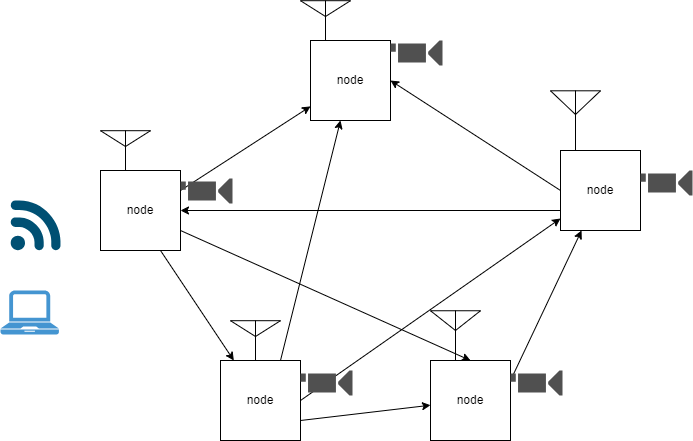
\includegraphics[width=0.5\linewidth]{Images/basic mesh network diagram.png}\par
	    \caption{Basic block diagram of a mesh network}
	
	    \label{Basic block diagram of a mesh network}
	     \end{center}
	\end{figure}
	each node will be attached to a tree  each having a transceiver